\documentclass[12pt,letterpaper,oneside]{book}

\usepackage{amsmath}
%\usepackage{amsthm}
\usepackage{algorithm}
\usepackage{algpseudocode}
\usepackage{esvect}
\usepackage{caption}
\usepackage{multirow}
\usepackage{hyperref}

%\usepackage[utf8]{inputenc}
\DeclareFixedFont{\ttb}{T1}{txtt}{bx}{n}{9} % for bold
\DeclareFixedFont{\ttm}{T1}{txtt}{m}{n}{9}  % for normal
% Defining colors
\usepackage{color}
\definecolor{deepblue}{rgb}{0,0,0.5}
\definecolor{deepred}{rgb}{0.6,0,0}
\definecolor{deepgreen}{rgb}{0,0.5,0}
\usepackage{listings}

\lstdefinestyle{Common}
{
    extendedchars=\true,
    language={[Visual]Basic},
    frame=single,
    %===========================================================
    framesep=3pt,%expand outward.
    framerule=0.4pt,%expand outward.
    xleftmargin=3.4pt,%make the frame fits in the text area. 
    xrightmargin=3.4pt,%make the frame fits in the text area.
    %=========================================================== 
    rulecolor=\color{Red}
}


\usepackage{./afitStyleFiles/afitThesis}
\usepackage{./afitStyleFiles/sf298}
\graphicspath{{./Figures/}}
\usepackage{tikz}
\usetikzlibrary{positioning}
\errorcontextlines 10000
\usepackage{enumitem}
\usepackage{amsmath}
\usepackage{adjustbox}
\usepackage{subfig}
\usepackage{tabularx}
\usepackage{url}
\usepackage{listings}
\usepackage{relsize} 
\usepackage{placeins}
\usepackage{url}





%emojis
\usepackage{graphicx}

%subsections
\usepackage{titlesec}
\setcounter{secnumdepth}{4}
\titleformat{\paragraph}
{\normalfont\normalsize\bfseries}{\theparagraph}{1em}{}
\titlespacing*{\paragraph}
{0pt}{3.25ex plus 1ex minus .2ex}{1.5ex plus .2ex}

%% Customize your document with your personal information
%% First, comment out the appropriate document type
\afitthesis %%default
%\afitreport
% \dissertation
% \prospectus

\author{Jocelin S. Maus}
\rank{Captain, USAF} % If a civilian, comment out this line.

\docdesignator{AFIT-ENS-MS-19-M-137}
\department{Department of Operational Sciences}
\graduationdate{March 2019}

\flytitle{Applying the Multiple Knapsack Assignment Problem to a Cargo Allocation and Transportation Problem with Stochastic Demand} 

       
\title{\MakeUppercase{Applying the Multiple Knapsack Assignment Problem to a Cargo Allocation and Transportation Problem with Stochastic Demand}}       
                             % Note, if you use \MakeUppercase to put
                             % the title in all uppercase as the style
                             % guide demands, understand that the
                             % command does not allow page breaks ``\\'' 
                             % within its brackets.
\previousdegrees{B.S.}
\acdegree{Master of Science in Operations Research}

\committee{{Maj Thomas P. Talafuse, Ph.D.\\Chair},
           {Lt Col Jeremy D. Jordan, Ph.D.\\Member},
           {Dr. Brian J. Lunday\\Member}}

\address{2950 Hobson Way\\ Air Force Institute of Technology \\
Wright-Patterson AFB, OH 45433}

\distribution{DISTRIBUTION STATEMENT A\\[-10pt]
\MakeUppercase{Approved for Public Release; distribution unlimited.}
}

\disclaimer{The views expressed in this document are those of the
author and do not reflect the official policy or position of the
United States Air Force, the United States Army, the United States
Department of Defense or the United States Government.  This 
material is declared a work of the U.S. Government and is not 
subject to copyright protection in the United States.}

% International students may consider using the following disclaimer
% statement: \dislaimer{The views expressed in this document are those
% of the author(s) and do not reflect the official policy or position
% of the United States Air Force, Department of Defense, United States
% Government, the corresponding agencies of any other government,
% NATO, or any other defense organization.}


%\input{Preamble/myFigures}		<--Will want to comment back in at some point
%\input{Preamble/commonSymbols}	<--Will want to comment back in at some point

%These don't work-- 
%\usepackage{indentfirst}
%\setlength{\parindent}{4em}

\definecolor{deepblue}{rgb}{0,0,0.5}
\definecolor{deepred}{rgb}{0.6,0,0}
\definecolor{deepgreen}{rgb}{0,0.5,0}

%\def\nopunct{\spacefactor 1007 }
%\def\frenchspacing{\sfcode`\.1006\sfcode`\?1005\sfcode`\!1004%
%\sfcode`\:1003\sfcode`\;1002\sfcode`\,1001 }

\begin{document}

%___________________________________
%Introductory Information

%\frontmatter
%	\flyleaf
 %   \disclaimerpage
%	\titlepageAFIT
%	\committeepage
 %   %\begin{abstract}
%Need to write

%\end{abstract}
  %  \begin{dedication}
 Dedication Section


\end{dedication}
  %  \begin{acknowledgements}

%\begin{quote}
%      \emph{If I have seen further, it is by standing on the shoulders of giants.}\\
%\end{quote}
%\begin{flushright}
%-- Sir Isaac Newton
%\end{flushright}




\end{acknowledgements}
  %  \tableofcontents
  %  \listoffigures
  %  \listoftables
\mainmatter


%___________________________________
%Chapter 1 -- Introduction
 \chapter{Introduction}\label{ch1}
  
\section{Background}
The US military relies on airlift to not only deploy and sustain U.S. armed forces anywhere in the world but also to rapidly mobilize humanitarian efforts and supplies.  A growing concern for the modern military budget is how to provide airlift functions expediently with economical awareness. Research on the subject of cargo transportation via aircraft has existed as long as the advent of military airlift itself. With it, a myriad of paths to improve cargo transportation have emerged.  Historically, to improve cargo throughput, aircraft designers emphasized larger and faster planes, however recently these efforts have plateaued.  New planes are marginally better than old in the realm of size and speed.  %The fleet of the United States Air Force's main cargo airlift provider, Air Mobility Command (AMC), is aging.  Currently, there are 52 C-5B/C/M, the newest of which was delivered to the Air Force in 1989 \cite{C5}.  Military expenditure in the near future will not be towards a new air mobility fleet (inferred from old DoD "The Mobility Capabilities and Requirements Study 2016 (MCRS-16)" published in 2009 new ). 
Recent considerations of the improvement of air transportation have delved into fuel efficiency. Reiman proposed improving fuel efficiency and cargo throughput through alternative routing methods \cite{Reiman2014}. Boone presented a methodology that incorporates ensemble, versus deterministic, numerical weather prediction models into route planning, thus reducing the
amount of excess fuel burned by poor forecasts and providing a range of potential values which aid in flight planning \cite{Boone2018}.    

\section{Motivation}

Optimization has been widely used in the civilian sector to save costs, promote efficiency, and reduce waste.  While government entities should endeavor to optimize for the same reasons, they also utilize optimization to conserve manpower, improve lethality, and save lives. Supplying troops and humanitarian aid is a military transportation problem.  %Travel on nonproductive legs diminishes the aircraft's productivity, and more often than not, cargo aircraft must fly one ormore positioning legs to an onload location \cite{AFPAM10-1403}.  
Operations already impacted by the limited capacity of aircraft also fall prey to dynamic requirements and differing priorities of multiple global locations.  The question is how to assign and utilize varying cargo aircraft types to these demands to minimize cost and maximize priority fulfillment.  %The inherent tradeoff is fulfilling demands now, with the possible loss of productivity of an aircraft, or waiting for future demands thus maximizing the productivity of the aircraft but not fulfilling all demands expediently. The priority of the demand, positioning of assets, capacity of aircraft, and transportation cost all affect this decision.
Solving the problem can be done through modeling the problem as an extension of the traditional knapsack problem and the assignment problem.  Chapter 2 reviews current methodologies for solving the multiple knapsack assignment problem as well as the foundational research to the all-inclusive approach to airlift planning in the Aircraft Selection Model (ASM) \cite{maywald}.

%``Fuel efficiency must be assessed simultaneously with cargo throughput which is the primary goal of airlift effectiveness." \cite{Reiman}



%___________________________________
%Chapter 2 -- Literature Review
\chapter{Literature Review}\label{ch2}
 

\section{Overview} 
This chapter discusses the multiple knapsack problem (MKP) and the assignment problem, as well as several hybridizations of exact and heuristic methods to solve each.  The traditional knapsack problem (KP) is a combinatorial optimization problem concerned with finding the optimal combination of \textit{j} out of $n$ items with values $p_j$ and weights $w_j$, to fill a ``knapsack" to maximize value without busting the knapsack capacity constraint, $c$ \cite{knapsackProblems}. 
\begin{align}
\begin{cases}
\max &\sum_{j=1}^n p_jx_j\\
\text{subject to} &\sum_{j=1}^n w_jx_j\leq c\\
&x_j \in \{0,1\} \text{,}	\hspace{5mm}\text{j=1,...,n}
\end{cases}
\end{align}

It is one of Karp's NP-Complete problems \cite{Karp2010ReducibilityProblems}. Approaches that compute optimal solutions for the KP are the use of dynamic programming and the branch and bound method. Both approaches can be time and memory consuming for trivial instances of the KP and are not practical.         
Approximation schemes solve the problem to optimality or close to optimality while saving time and memory.
Recent research by Haddar \textit{et al.} \cite{Haddar2016} uses an evolutionary computation technique, the Quantum Particle Swarm Optimization (QPSO), with a local search method in order to solve the KP. 
The KP has many real life applications other than bag packing, such as cutting stock, capital budgeting, and cryptography \cite{Wilbaut2008}.  Kosuch and Lisser \cite{Kosuch2011OnProblems} studied a particular instance of a stochastic knapsack where items of unknown weight are assigned to knapsacks in a first stage and can be taken out or added to the knapsack after a second stage, when the actual weights become known. They proved that when searching for good lower bounds, one can replace an exhaustive branch-and-bound framework
by a heuristic.  Perry and Hartman \cite{Perry2009} modeled a case of a stochastic dynamic knapsack, where items arrive according to a stochastic process and stay in the knapsack for a number of time periods before exiting. Ross and Tsang \cite{Ross1989} applied the concept of a stochastic dynamic knapsack to bandwidth allocations of communications switching network to randomly arriving calls of random length.        

%A special case of a KP, known as a multidimensional knapsack problem, seeks to find a subset of items that maximizes a linear objective function while satisfying a set of linear capacity constraints.

\section{Multiple Knapsack}
The multiple knapsack problem is an extension of the KP problem where there are \textit{n} items and \textit{m} knapsacks $(m\leq n)$. When $m=1$, a MKP reduces to the traditional KP problem \cite{MKPChapter}. 

\begin{align}
\begin{cases}
\max 				&\sum_{i=1}^m\sum_{j=1}^n p_jx_{ij} \\
\text{subject to}   &\sum_{j=1}^n w_jx_{ij}\leq c_i \text{,}	 \hspace{5mm}\text{i=1,...,m}\\
					&\sum_{i=1}^m x_{ij}\leq 1 		\text{,} 	 \hspace{5mm}\text{j=1,...,n}\\
					&x_{ij} \in \{0,1\} 				\text{,} \hspace{5mm}\text{i=1,...,m} \text{,}	 \hspace{5mm}\text{j=1,...,n}
\end{cases}
\end{align}

The first MKP was published by Eilon and Christofides \cite{EilonChristofides1971} in 1971 as a loading problem ``defined as the allocation of items with known magnitude to boxes with constrained capacity so as to minimize the number of boxes required" \cite{EilonChristofides1971}.  The recommended solutions were to use a zero-one programming model and a heuristic.  The heuristic involved a cycle of scanning for items to precisely fill boxes and performed well compared to the zero-one programming method, finding the optimal solution to 48 out of 50 problems in significantly less computing time in comparison.  More recently, Lai \textit{et al.} \cite{Lai2018} innovated an effective hybrid evolutionary algorithm using a solution-based tabu search for solving the MKP. As of 2017, their algorithm reproduced the best known results for the vast majority of instances tested and established new best known solutions, or improved lower bounds, for four hard instances.  To solve a dynamic, stochastic MKP, Perry and Hartman \cite{Perry2009} presented a stochastic dynamic program (SDP) recursion. Their approximation approach utilizes simulation and deterministic dynamic programming  to allow for the solution of longer horizon problems and ensure good time zero decisions. 
Solutions to the MKP can aid in more than answering physical allocation issues; Simon \textit{et al.} \cite{Simon2017} applied the MKP to assess the different factors that impact Marine self-sufficiency.

\section{Multidimensional Knapsack}
Differing from the multiple knapsack, the multidimensional knapsack problem is an extension of the KP problem where there are multiple resource constraints or a constraint with a multidimensional attribute \cite{knapsackProblems}. 
\begin{align}
\begin{cases}
\max &\sum_{j=1}^n p_jx_j\\
\text{subject to} &\sum_{j=1}^n w_{ij}x_j\leq c_i \hspace{5mm}\text{i=1,...,d}\\
&x_j \in \{0,1\} \text{,}	\hspace{5mm}\text{j=1,...,n}
\end{cases}
\end{align}
\cite{Shih1979AProblem}

\section{Assignment Problem} A transportation problem has a goal of determining the minimal cost to move a product through a bipartite network in order to satisfy demands at one half of the network from available supplies at the other half. \cite{ahuja} The assignment problem is a balanced transportation problem where the goal is to minimize the cost of matching supply and demand so that each supply is only matched to one demand and vice versa \cite{Winston2004OperationsAlgorithms}. 
%
\begin{align}
\begin{cases}
\min 				&\sum_{i=1}^m\sum_{j=1}^n cost_{ij}x_{ij} \\
\text{subject to}   &\sum_{j=1}^n x_{ij}= 1 \text{,}	 \hspace{5mm}\text{i=1,...,m}\\
					&\sum_{i=1}^m x_{ij}= 1 		\text{,} 	 \hspace{5mm}\text{j=1,...,n}\\
					&x_{ij} \in \{0,1\} 				\text{,}	 \hspace{5mm}\text{i=1,...,m}\text{,}	 \hspace{5mm}\text{j=1,...,n}
\end{cases}
\end{align}

Ram Vaswani \cite{vaswani} originally applied the assignment problem to the allocation of cargo to aircraft. In the aircraft assignment problem, Vaswani used the Hungarian algorithm to assign one of ten types of cargo to one of ten aircraft, with a pre-calculated aircraft-cargo assignment cost provided in matrix form.  Ferguson and Dantzig \cite{ferguson_dantzig_aircraftRouting} illustrated an application
of linear programming to the problem of assigning aircraft
to routes to maximize profits and later expanded upon the problem to maximize expected profits when there is
uncertain customer demand \cite{ferguson_dantzig_uncertainDemand}. Wu and Ross \cite{WuRoss2014} investigated a case of a stochastic assignment problem where balls arrive sequentially (as demands would arrive over a period of time) and need to be assigned to boxes  to minimize arrivals, \textit{N}.  A ball only fits in certain types of boxes, and the types it can fit in is not known until arrival. The solution to Wu and Ross's stochastic assignment problem involves a heuristic policy to minimize the expected number of arrivals and a dynamic program to improve upon the heuristic policy.       

\section{Multiple Knapsack Assignment Problem}
The multiple knapsack assignment problem (MKAP) is an extension of the MKP and of the assignment problem where \textit{n} items are broken into \textit{K} mutually disjoint subsets of items and the goal is to assign knapsacks to each subset and solve to maximize the total profit of accepted items. 
\begin{align}
\begin{cases}
\max 				&\sum_{i=1}^m \sum_{k=1}^K\sum_{j\in N_k} p_jx_{ij} \\
\text{subject to}   &\sum_{j\in N_k} w_jx_{ij}\leq c_iy_{ik} \text{,}	 \hspace{5mm}\text{i=1,...,m}\text{,}	 \hspace{5mm}\text{k=1,...,K}\\
					&\sum_{i=1}^m x_{ij}\leq 1 		\text{,} 	 \hspace{5mm}\text{j=1,...,n}\\
                    &\sum_{k=1}^K y_{ij}\leq 1 	\text{,} 	 \hspace{5mm}\text{i=1,...,m}\\
					&x_{ij},y_{ij} \in \{0,1\} 	\text{,}	 \hspace{5mm}\forall i,j,k
\end{cases}
\end{align}
%
Kataoka and Yamada \cite{Kataoka2014} first introduced the problem in 2014 and presented a heuristic algorithm to solve this problem approximately as well as three ways to compute the same upper bound.  Their solution method for the MKAP uses a greedy heuristic to assign the subsets, performs a local search to improve the results, and then decomposes the problem into \textit{K} MKPs. Feasible solutions to the MKPs are truncated to save time and to approximate the lower bound. Dimitrov \textit{et al.} \cite{Dimitrov2017EmergencyProblem} presents special cases of the MKAP regarding emergency relocation of items and the formulation of the MKAP when items to be assigned to knapsacks are identical or of equal value. 

\section{Branch-and-Bound Method}
The branch-and-bound method is the repeated partitioning of a solution space into subspaces, solving for the objective value in the subspaces, and decreasing the search space if subspace values are suboptimal. The term \textit{branch} refers to the partitioning of the problem, and \textit{bound} refers to the determination of the solution and therefore the boundary of the subspace. This method utilizes relaxation on constraints to initialize upper and lower bounds for the global optimal solution.  If a new branch's solution is outside of these bounds, then it is not considered for further exploration.  A successful iterative process of the branch and bound method will converge to a global optimal solution. \par 
 William Cook \cite{Cook2012MarkowitzBound} found that the method was proposed in the late 1950s by several individuals. In 1957 Harry Markowitz and Alan Manne described the components of the branch and bound method and a general approach, but did not present an automatic algorithm for solving. Willard Eastman, in his 1958 Ph.D. dissertation (cited in \cite{Cook2012MarkowitzBound}), also used the concept of establishing bounds to eliminate the investigation of branches, however it was not until 1960 that Ailsa Land and Alison Doig \cite{Land2010AnProblems} presented the numerical algorithm for the branch and bound method. John Little, Katta Murty, Dura Sweeney, and Caroline Karel \cite{Little1963AnProblem} coined the term ``branch and bound" in their 1963 paper on solving the traveling salesman problem. \par
 \section{BARON}
The branch and bound method is highly utilized today for solving combinatorial and mixed integer problems. Many mathematical program solvers use algorithms of the brand and bound method as the foundation of the program's processing.  The Branch-And-Reduce Optimization Navigator (BARON) is one computational system that implements algorithms of the branch-and-bound type to find the global solution of algebraic nonlinear programs (NLPs) and mixed-integer nonlinear programs (MINLPs). BARON requires bounds on variables and nonlinear expressions in the mathematical program \cite{BARON_UserManual}, and utilizes feasibility reduction, duality reduction, and a learning heuristic \cite{Tawarmalani2004GlobalStudy} to reduce the range of the solution region until optimality is attained. A high level visual of the BARON algorithm may be seen in figure \ref{fig_BARON}.   

\begin{figure}[H]
\centering
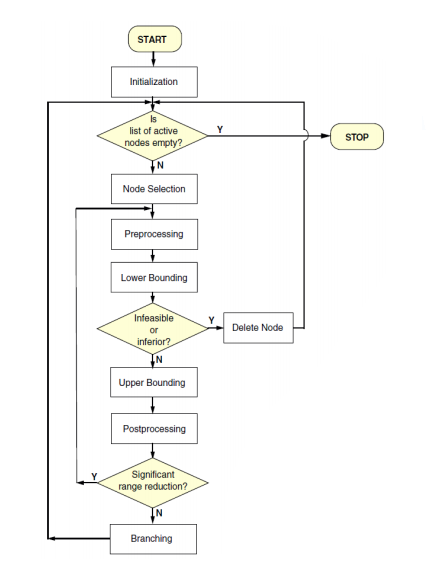
\includegraphics[width=85mm]{Algorithm_BARON.PNG}
\caption{BARON Algorithm \cite{Lipp2011BARONCME334}}
\label{fig_BARON}
\end{figure}

To solve the subproblems, BARON calls upon other solvers. By default, BARON utilizes CPLEX for linear problems and MINOS for nonlinear problems. CPLEX generally solves linear problems using the dual simplex algorithm. For problems with a nonlinear objective MINOS solves for local optima using a reduced gradient algorithm combined with a quasi-Newton algorithm. For problems with nonlinear constraints MINOS solves for local optima by using a projected Lagrangian algorithm. The program iterates through subproblems with linearized versions of the constraints and utilizes the reduced-gradient algorithm to solve \cite{GAMS_old}. 
\section{Aircraft Routing and Resources}
In \cite{Reiman2014} Reiman developed regression equations on flight data from aircraft performance manuals to estimate the fuel consumption required of the C-5, C-17, or the C-130 to climb, cruise and descend based on the aircraft gross weight, altitude and distance to travel. 
These mathematical models, in addition to a nodal reduction heuristic, were utilized to generate fuel efficient route alternatives for the strategic airlift problem. Follow-on research \cite{maywald} showed that fuel efficiency and cargo throughput can be improved using this alternative route method and the concept of hopping, compared to current cargo routes. Hopping is when an aircraft makes enroute stops to refuel thus allowing aircraft to carry more in payload weight instead of fuel weight to get to the destination \cite{Nangia2006OperationsRefuelling}. Extra stops require time, resource availability at enroute airfields of crews and aircraft maintenance, and the premise of hopping relies upon capitalizing on the fuel efficiency of smaller aircraft. While Maywald \textit{et. al.} \cite{maywald} do not account for resource availability, Baker \textit{et. al.} \cite{Baker2002OptimizingAirlift} evaluated the requirements for airfield resources to meet aircraft demand, including aircraft specific maintenance, ramp space and fuel pumping rates. 

%___________________________________
%Chapter 3 -- Methodology
  \chapter{Methodology}\label{ch3}
   \section{Introduction}
This chapter outlines the methodology for the multiple knapsack assignment problem approach utilized in this research. Described in depth are the fuel estimation equations and the distance formula used in the model. Then the mathematical model is outlined. Lastly detailed are how the model inputs are prepared and the solution is processed.

\section{Fuel Estimation} \label{sec_fuelEquations}
In \cite{Reiman2014} Reiman developed fuel regression equations based on flight data from aircraft performance manuals for the C-17, C-5, and C-130.  These equations model the fuel, in kilo-pounds, required of the three aircraft types to climb, cruise and descend based on the aircraft gross weight, altitude and distance to travel.  While the equations allow for a user-defined altitude, the analysis was based on using the optimal cruise altitude for an aircraft's maximum gross takeoff weight. These aircraft assumptions are listed in Table \ref{tableAssume}.  
\begin{table}[h!]
\centering
\caption{Aircraft Specific Payload Movement Assumptions \cite{Reiman2014}}
\label{tableAssume}
\begin{tabular}{@{}lccc@{}}
\toprule
 & C-5 & C-17 & C-130 \\ \midrule
Operating Weight $\omega_{op}$ & 380 & 282.5 & 78 \\
Max Gross Takeoff Weight $\omega_{mgt}$ & 769 & 585 & 155 \\
Fuel Capacity $\omega_{fcap}$ & 347 & 241.36 & 62 \\
Aircraft Max Payload, $\omega_{apmax}$ & 270 & 170.9 & 53 \\
Reserve Fuel $\omega_{frc}$& 23.45 & 21.44 & 4 \\
Alternate Fuel \} $\omega_{fah}$ & 23.45 & 21.44 & 4 \\
Holding Fuel  & 17.59 & 16.08 & 0 \\
Start Taxi Takeoff Fuel $\omega_{fstto}$ & 3 & 4.5 & 0.67 \\
Approach $\omega_{fapp}$ & 7 & 2.67 & 0.7 \\ \bottomrule
\end{tabular}
\end{table}


Values for each regression model depend on the weights from Table \ref{tableAssume} as well as calculated values from one or both of the other regression models.  The combination of given weights from Table \ref{tableAssume} and the calculated weights result in Equation \ref{eq_fuel_ramp} for the ramp fuel weight. Equation  \ref{eq_fuel_ramp} plays a part in Equation \ref{eq_fuel_climb}, the model calculating the fuel required to climb.  The regression coefficient values for the climb equation are in Table \ref{tableClimb}. The regression coefficient values in Table \ref{tableDescent} are for Equation \ref{eq_fuel_descent}, the model calculating the fuel required to descend.  \newline
\begin{equation}
\label{eq_fuel_ramp}
\omega_{rf}=\omega_{fstto}+\omega_{fc}+\omega_{ff}+\omega_{fd}+ \omega_{fapp}+\omega_{frc}+\omega_{fah}
\end{equation}
% \begin{equation}
% \label{eq_grossweight_descent}
% \omega_{gd}= \omega_g-\omega_{fstto}-\omega_{fc}-\omega_{ff}
% \end{equation}   
\begin{equation}
\label{eq_fuel_climb}
\omega_{fc}=\beta_0+\beta_1\alpha+\beta_2\alpha^2+\beta_3\alpha^3+\beta_4\omega+\beta_5\omega^2+\beta_6\omega^3+10^{-6}\beta_7\alpha^2\omega^3+10^{-6}\beta_8\alpha^2\omega^3
\end{equation}
\begin{equation}
\label{eq_fuel_descent}
\omega_{fd}=\beta_0+\beta_1\omega_{gd}+\beta_2\omega_{gd}^2+\beta_3\alpha+\beta_4\alpha\omega_{gd}
\end{equation}
\setlength{\jot}{-1ex}
\renewcommand*\arraystretch{.8}
where:
\begin{align*}
\omega_{fc} &= \text{Fuel to Climb in Klbs}\\
\omega_{fd} &= \text{Fuel to Descend in Klbs}\\
\alpha &= \text{Altitude in Thousands of Feet}\\
\omega &=\text{Aircraft Gross Weight in Klbs at Climb Start}\\
&=\omega_{rf}+\omega_{op}+\omega_p\\
\omega_{gd} &=\text{Aircraft Gross Weight in Klbs at Descent Start}\\
&= \omega-\omega_{fstto}-\omega_{fc}-\omega_{ff}\\
\omega_{fstto} &= \text{Fuel for Start, Taxi, and Takeoff in Klbs}\\
\omega_{ff} &=\text{Fuel to Cruise in Klbs}
\end{align*}
%
\begin{table}[h!]
\begin{minipage}{.5\linewidth}
\centering
\caption{Climb $\omega_{fc}$ Regression Terms \cite{Reiman2014}}
\label{tableClimb}
\begin{tabular}{@{}lccc@{}}
\hline
\hline
& C-5  & C-17 & C-130\\\hline
$\beta_0$ & -3.0115 & -4.7054 & -1.067 \\
$\beta_1$ & 0.3192 & 0.2869 & 0.0669 \\
$\beta_2$ & -0.0082 & -0.007 & -0.0022 \\
$\beta_3$ & 9.50E-05 & 7.10E-05 & 3.00E-05 \\
$\beta_4$ & 0.0164 & 0.0267 & 0.0218 \\
$\beta_5$ & -3.30E-05 & -5.90E-05 & -0.0002 \\
$\beta_6$ & 2.20E-08 & 4.80E-08 & 5.20E-07 \\
$\beta_7$ & 3.70E-05 & 6.70E-05 & 0.0003 \\
$\beta_8$ & 7.10E-08 & -2.10E-07 & 1.30E-05\\ \hline
\end{tabular}
\end{minipage}
\begin{minipage}{.5\linewidth}
\centering
\caption{Descent $\omega_{fd}$ Regression Terms \cite{Reiman2014}}
\label{tableDescent}
\begin{tabular}{@{}lccc@{}}
\hline
\hline
& C-5  & C-17 & C-130\\\hline
$\beta_0$ & -1.9673 & 0.2574 & -0.0513 \\
$\beta_1$ & 0.0128 & 0.0005 & -0.0012 \\
$\beta_2$ & 1.34E-05 & -8.50E-07 & 1.38E-05 \\
$\beta_3$ & 0.1254 & 0.0108 & 0.0367 \\
$\beta_4$ & 0.0004 & 3.20E-05 & -0.0002\\\hline
\end{tabular}
\end{minipage}
\end{table}

\pagebreak The regression coefficient values for Equation \ref{eq_fuel_cruise}, the model calculating the fuel required to cruise, are in Table \ref{tableCruise}. While the weight of the reserve fuel and the alternate fuel are not planned to be consumed, they are a necessary part in the fuel equations because they add to the overall ramp fuel weight and weight of the plane over the course of the flight.

\setlength{\jot}{+1ex}
\begin{equation}
\label{eq_fuel_cruise}
\begin{aligned}
\omega_{ff}=&-\frac{B}{3A}-\frac{1}{3A} \sqrt[3]{\frac{1}{2}[2B^3-9ABC+27A^2D+\sqrt[]{(2B^3-9ABC+27A^2D)^2-4(B^2-3AC)^3]}}\\
&-\frac{1}{3A}\sqrt[3]{\frac{1}{2}[2B^3-9ABC+27A^2D-\sqrt[]{(2B^3-9ABC+27A^2D)^2-4(b^2-3AC)^3}]}
\end{aligned}
\end{equation}


\setlength{\jot}{-1ex}
 where (all weights in Klbs):\\
 $A =\frac{\beta_4}{3}\\$
 $B =(\frac{\beta_3}{2}+\beta_4(\omega_{op}+\omega_{frc}+\omega_{fah}+\omega_p)+\frac{\beta_5}{2}\alpha)$\\
 $C=\beta_0+\beta_1\alpha+\beta_2\alpha^2+\beta_3(\omega_{op}+\omega_{frc}+\omega_{fah}+\omega_p)+$\\
 \text{\hspace{9mm}}$\beta_4(\omega_{op}+\omega_{frc}+\omega_{fah}+\omega_p)^2+\beta_5\alpha(\omega_{op}+\omega_{frc}+\omega_{fah}+\omega_p)$\\
 $D= -\delta$\\
 $\delta = \text{Distance in NMs}$\\
% $\omega = \text{Aircraft Gross Weight}$\\
 %\text{\hspace{5mm}}$=\omega_{op}+\omega_{frc}+\omega_{fah}+\omega_p+f$\\
 $\omega_{op} = \text{Operating Weight}$\\
 $\omega_{frc}=\text{Reserve/Contingency Fuel Weight}$\\
 $\omega_{fah}=\text{Alternate/Holding Fuel Weight}$\\
 $\omega_p= \text{Payload Weight}$\\
 %$f= \text{Fuel Consumed}$\\
 $\omega_{ff}= \text{Fuel to Cruise in Klbs}$\\
 \setlength{\jot}{+1ex}


\begin{table}[h!]
\centering
\caption{Cruise $\omega_{ff}$ Regression Terms \cite{Reiman2014}}
\label{tableCruise}
\begin{tabular}{@{}lccc@{}}
\hline
\hline
 & C-5 & C-17 & C-130 \\ \hline
$\beta_0$ & 24.538 & 31.735 & 58.829 \\
$\beta_1$ & 0.5511 & 0.9897 & 3.5292 \\
$\beta_2$ & 0.0002 & -0.0043 & -0.0098 \\
$\beta_3$ & -0.0318 & -0.0642 & -0.2384 \\
$\beta_4$ & 0.000019 & 0.000058 & 0.001 \\
$\beta_5$ & -0.0005 & -0.0011 & -0.0155
\end{tabular}
\end{table}

\section{Distance Estimation}
The solution to this application of the MKAP relies heavily on Reiman's \cite{Reiman2014} fuel estimation equations. One factor in these equations is distance. Utilized in both Reiman's work and in this research is the Vincenty distance formula \cite{Vincenty1975DirectEquations}. Instead of assuming a straight line distance and using the Pythagorean Theorem, or assuming a spherical Earth and using the great-circle distance, the Vincenty Inverse Method assumes the Earth is a flattened spheroid and iteratively calculates distance via ellipsoidal geometry given the latitude and longitude of both the source and the destination points.  The reference used for Earth's geospatial properties in Reiman's and this work is the World Geodetic System 1984 (WGS84) \cite{WGS}.\par
The maximum distance an aircraft can traverse is estimated assuming that cruise and descent fuel have little impact on distance. Equation \ref{eq_fuel_cruise} is used, setting the fuel consumed equal to the maximum amount of fuel an aircraft is allowed to carry given a payload weight, Equation \ref{eq_maxFuel}, and solving for distance.
\begin{equation}
\label{eq_maxFuel}
maxFuel=min(\omega-\omega_{op}-\omega_p, \hspace{3mm} \omega_{fcap}) 
\end{equation}
\newpage
\section{Mathematical Model} \label{sec_mathModel}
The mathematical program for the problem uses the fuel equations in not only the constraints, but also the objective function, Equation \ref{eq_obj}.  There are two sets of bases, one acting as a supplier and one as the demand. Expected demand is used as the constraint in Equation \ref{eq_demand} for the amount required to be sent to the demanding base from all suppliers. The aircraft is a largely constraining factor in the problem. Each aircraft has a maximum weight for payload, takeoff, and fuel, shown in Table \ref{tableAssume} and accounted for in Equations \ref{eq_payloadCap}, \ref{eq_maxGrosstakeoff}, \ref{eq_fuelCap}, respectfully. Aircraft also have a given amount of floor space for cargo \cite{C5}\cite{c-17}\cite{c130}, therefore the amount of cargo cannot exceed the given floor space in Equation \ref{eq_spaceCap}. Cargo is assumed to be on standard pallets, and is constrained to the properties associated with a standard pallet of item type $K$ in Equation \ref{eq_IntegerPAllets}; there are no partial pallets. A supplying base has a limit on the number of a specific item type $K$, and is only allowed to send what is available in inventory in Equation \ref{eq_supplyconstraint}. Equations \ref{eq_AC_Assignment} and \ref{eq_binaryAssignment} are the assignment equations, ensuring an aircraft is only allowed to fly the cargo between one supply-demand pairing.\\  

\textbf{Sets:}\newline
$I$  set of supply bases, indexed by $i$\\
$J$  set of demand bases, indexed by $j$\\
$K$  set of item types, indexed by $k$\\
$L$  set of aircraft, indexed by $l$\newline

\textbf{Decision Variables:}  \newline
$x_{ij}^{kl}$  number of pallets of item $k$ to fly on aircraft $l$ from base $i$ to base $j$.  \newline
$y_{ij}^l$  assignment of aircraft $l$ to deliver from base $i$ to base $j$.  \newline

\textbf{Parameters:} \newline  
$D_j^{k}$  expected demand of base $j$ for item $k$   \newline 
$supply_i^k$  supply inventory of item $k$ at base $i$   \newline 
$w_{k}$  weight of item type $k$  \newline 
$\omega_{mgt}^{l}$ maximum gross takeoff weight for aircraft $l$   \newline
$\omega_{apmax}^l$ maximum payload weight for aircraft $l$ \newline
$\omega_{fcap}^l$ maximum fuel weight for aircraft $l$ \newline
$\omega_{rf}^l$ ramp fuel weight for aircraft $l$ \newline
$\omega_{frc}^l$ reserve/contingency fuel weight for aircraft $l$ \newline
$\omega_{fah}^l$ alternate/holding fuel weight for aircraft $l$ \newline
$f_{ij}^l$ total fuel consumed in Klbs, $f=\omega_{rf}-\omega_{frc}-\omega_{fah}$ \newline
$space^{l}$  space capacity of cargo floorspace of aircraft type $l$   \newline 
$fuelPrice$ current market price of fuel per Klb\\ 
\newpage
\textbf{Objective Function:}  
\begin{equation}
\label{eq_obj}
\min \hspace{5mm}
fuelPrice*\sum_{i\in I}\sum_{j\in J}\sum_{l\in L}(f_{ij}^l|y_{ij}^l \text{ and } x_{ij}^{kl}) 
%(\omega_{fstto}^{l}+\omega_{fc}^{ijl}+\omega_{ff}^{ijl} + \omega_{fd}^{ijl}+\omega_{app}^{l})
\end{equation}

\textbf{Subject to:}
\begin{align}
\sum_{i\in I}\sum_{l\in L}x_{ij}^{kl}&= D_j^{k} &\forall \hspace{2mm} j \in J \text{, } k\in K \label{eq_demand}\\
\sum_{k\in K}w_{k}x_{ij}^{kl}&\leq \omega_{apmax}^{l}y_{ij}^l &\forall \hspace{2mm} i \in I \text{, } j\in J \text{, } l \in L \label{eq_payloadCap}\\
\omega_{g}^{ijl}&\leq \omega_{mgt}^l &\forall \hspace{2mm} i \in I \text{, } j\in J \text{, } l \in L \label{eq_maxGrosstakeoff}\\
\omega_{rf}^{ijl} &\leq \omega_{fcap}^l &\forall \hspace{2mm} i \in I \text{, } j\in J \text{, } l \in L \label{eq_fuelCap}\\
\sum_{k\in K}x_{ij}^{kl} &\leq space^{l}y_{ij}^l  &\forall \hspace{2mm}  i\in I \text{, } k\in K \text{, } l\in L \label{eq_spaceCap}\\
\sum_{j\in J}\sum_{l \in L}x_{ij}^{kl} &\leq supply_i^k &\forall\hspace{2mm} i \in I \text{, } j\in J \label{eq_supplyconstraint}\\
x_{ij}^{kl}& \text{  integer}  \hspace{15mm}&\forall \hspace{2mm} i\in I \text{, } j \in J \text{, } k\in K \text{, } l \in L \label{eq_IntegerPAllets}\\ 
\sum_{i \in I}\sum_{j\in J}y_{ij}^l &\leq 1 &\forall \hspace{2mm} l \in L \label{eq_AC_Assignment}\\
y_{ij}^l &\in \{0,1\} &\forall \hspace{2mm} i \in I \text{, } j \in J \text{, } l\in L \label{eq_binaryAssignment}
\end{align}

\pagebreak
\section{Assumptions} \label{sec_assumptions}
Several assumptions were made in the interest of simplifying the computational complexity of the model.  While there are many bases which can act as supply and demand bases, the pavement of supply and demand locations sampled for this problem can handle the take-off and landing of any of the three types of aircraft with their respective maximum payloads.  Aircraft
maximum payload weight, maximum gross takeoff weight and operating weight are assumed to
be fixed as shown in Table \ref{tableAssume}.\par
It is assumed airfields are available for routing of aircraft, however, enroute stops are not calculated based on actual base locations, but are equidistant points on the direct route between supply demand pairings.  The necessity of one or more enroute stops for a given mission design series (MDS) and payload is calculated in Algorithm \ref{alg_numStops}. The number of stops is determined by dividing the Vincenty distance \cite{Vincenty1975DirectEquations} by the calculated maximum distance the aircraft can fly carrying the payload and rounding this number down to the closest integer. For example, if the distance between the pairings is less than the maximum distance at maximum payload weight, then the ratio would be less than one. This rounds down to a necessity of zero enroute stops.  No cargo is delivered or exchanged at enroute stops, however fuel tanks are re-filled to maximum capacity.\par
\begin{algorithm}[H]
\caption{Number of Stops}
\label{alg_numStops}
\begin{algorithmic}
\Function {numStops}{MDS, distance, payload}
		\State $numberStops =$ numStops(selectMDS, distance, payload)
        \State $stopDist =$ maxDistance(payload)
    	\State $numStops = roundDown(distance / stopDist)$
\EndFunction
\end{algorithmic}
\end{algorithm}
Demand bases do not have inventory restriction and have the equipment necessary to receive and handle any items. Weather is not a limiting factor and is not taken into account for routing or fuel cost. Reserve, contingency, alternate and holding fuels are safety fuels that are carried but not consumed.  The model assumes that aircraft are prepositioned to fulfill assignment pairings, and need not fly from another location to get to the supply base. The cost of prepositioning aircraft at supply locations is not a factor. Time is also not a factor.  There are adequate crew to fulfill the flight requirements of assignments. 

\section{Math Model Modifications} \label{sec_mathModelMod}
Complications implementing the fuel calculations within the General Algebraic Modeling System (GAMS) resulted in a modification to the mathematical model in the GAMS program. The objective function that drives the solution in GAMS was altered to solve minimizing an approximation to the fuel cost. Prior to running the GAMs model, the fuel cost of a specific aircraft flying from one supply location to one demand location is calculated for the plane carrying the maximum payload as well as the base fuel cost for flying no payload, Equation \ref{eq_baseFuelCost}. The cost per payload kilopound is calculated in Equation \ref{eq_costPerPayload} by taking the difference between these two values and dividing it by the maximum payload weight for the specific aircraft.
\begin{equation}
\label{eq_baseFuelCost}
baseFuelCost_{ij}^l=f_{ij}^l(zeroPayload)
\end{equation}
\begin{equation}
\label{eq_costPerPayload}
fuelCost_{ij}^l=\frac{f_{ij}^l(maxPayload)-baseFuelCost_{ij}^l}{\omega_{apmax}^l}
\end{equation}

Multiplying the payload by the cost per payload and adding it to the cost of flying the aircraft while empty results in the approximated cost of carrying the payload that is used in the GAMS objective function, Equation \ref{eq_obj2}. By altering the objective function from Equation \ref{eq_obj} to Equation \ref{eq_obj2}, the GAMS model no longer requires constraint Equations \ref{eq_maxGrosstakeoff} or \ref{eq_fuelCap}. Finally, to focus on the aspect of demand in the analysis, supply is assumed to be unlimitied, therefore the supply constraint, Equation \ref{eq_supplyconstraint}, is also removed.
\begin{equation}
\label{eq_obj2}
\min \hspace{5mm}
fuelPrice*\sum_{i\in I}\sum_{j\in J}\sum_{k\in K}\sum_{l\in L}(w_{k}x_{ij}^{kl}*fuelCost_{ij}^{l}+baseFuelCost_{ij}^l)
\end{equation}
\textbf{Subject to:}
\begin{align*}
\sum_{i\in I}\sum_{l\in L}x_{ij}^{kl}&= D_j^{k} &\forall \hspace{2mm} j \in J \text{, } k\in K \tag{\ref{eq_demand}}\\
\sum_{k\in K}w_{k}x_{ij}^{kl}&\leq \omega_{apmax}^{l}y_{ij}^l &\forall \hspace{2mm} i \in I \text{, } j\in J \text{, } l \in L \tag{\ref{eq_payloadCap}}\\
\sum_{k\in K}x_{ij}^{kl} &\leq space^{l}y_{ij}^l  &\forall \hspace{2mm}  i\in I \text{, } k\in K \text{, } l\in L \tag{\ref{eq_spaceCap}}\\
x_{ij}^{kl}& \text{  integer}  \hspace{15mm}&\forall \hspace{2mm} i\in I \text{, } j \in J \text{, } k\in K \text{, } l \in L \tag{\ref{eq_IntegerPAllets}}\\ 
\sum_{i \in I}\sum_{j\in J}y_{ij}^l &\leq 1 &\forall \hspace{2mm} l \in L \tag{\ref{eq_AC_Assignment}}\\
y_{ij}^l &\in \{0,1\} &\forall \hspace{2mm} i \in I \text{, } j \in J \text{, } l\in L \tag{\ref{eq_binaryAssignment}}
\end{align*}

\section{Solution Pre-processing} \label{sec_solutionPreProcessing}
Many of the subroutines and functions, written in Microsoft Excel Visual Basic for Applications (VBA), are used for data collection and pre-processing. Initially, the user is prompted to select the supply and demand airfields from a list of 5342 airfields from the Digital Aeronautical Flight Information File (DAFIF) database. The user may manually add the specific International Civil Aviation Organization airport code (ICAO) to the supply base list, or they may use a button to populate the list with the known channel continental United States (CONUS) supply bases, or, for completely proof of concept purposes, the user may use a button to randomly populate the list with a specific number of supply bases. With the selection of airfields the user is requested to input the inventory of the supply bases and the requirements for the demand bases of two cargo types, high priority, ``Priority 1" or ``Super/999/1," cargo and regular priority, ``Priority 2/3" cargo. They may do this manually, or may use a button on the respective pages to randomly populate the supply and demand. Up to this point, a supply sheet and a demand sheet have been created. Lastly, the user is asked to add the number of available C-5Bs, C17s, and C-130J-30s via the aircraft selection form, seen in Figure \ref{fig_acSelectionForm}. \par
\begin{figure}[H]
\centering
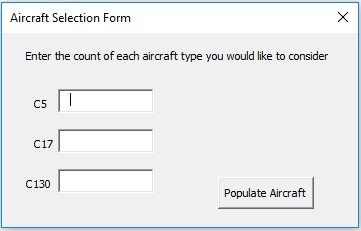
\includegraphics[width=80mm]{acSelectionForm.PNG}
\caption{Aircraft Selection Form}
\label{fig_acSelectionForm}
\end{figure}
Upon clicking the ``Populate Aircraft'' button, many subroutines and functions are called upon to create the aircraft page. This lists available aircraft, their associated parameters such as maximum takeoff weight and fuel capacity, and the calculated aircraft costs per payload and baseline fuel costs to fly between the source and destination pairings. The main subroutine called to perform this page creation is called GetDistance. As seen in Algorithm \ref{alg_getDistance}, the GetDistance subroutine initially finds the latitude and longitude for the supply base, then iterates through the demand bases. For each demand base, the latitude and longitude is found, then the program iterates through all available aircraft. The vincentyDistance function is called to calculate the Vincenty distance between the supply and demand base and fuel function is called to calculate the fuel cost given the distance, MDS, and payload.  For the base fuel calculation the payload is zero. For the max fuel calculation the payload is the maximum payload for the given aircraft type.\par
\begin{algorithm}[H]
\caption{Sub Routine GetDistance}
\label{alg_getDistance}
\begin{algorithmic}
\For{each supply base $i\in I$}
	\For{all $airfields$}
    	\If {$airfield=supply base$}
          	\State $lat1=airfield.latitude$
            \State $long1=airfield.longitude$
            \State \textbf{exit for} all airfields
        \EndIf
	\EndFor
    \For{each demand base $j\in J$}
		\For{all $airfields$}
			\If {$airfield=supply base$}
				\State $lat2=airfield.latitude$
            	\State $long2=airfield.longitude$
                \State $distance=$ vincentyDistance(lat1, long1, lat2, long2)
                \For {all aircraft $l \in L$} 
                	\State $MDS= aircraft.MDS$
                    \State $maxPayload=aircraft.maxpayload$
					\State $baseFuel=$fuel(MDS, distance, payload=0)
					\State $payloadFuel=$ fuel(MDS, distance, payload=maxpayload)
					\State $maxFuel= (payloadFuel-baseFuel)/maxPayload$
                	\State \textbf{write} supplyBase, demandBase, baseFuel, maxFuel 
                \EndFor
                \State \textbf{exit for} all airfields
        	\EndIf
      	\EndFor
	\EndFor
 \EndFor
\end{algorithmic}
\end{algorithm}
As seen in Algorithm \ref{alg_fuel}, the fuel function calls upon the numStops function to provide the number of stops the aircraft requires given payload and distance and calls upon the fuelCalculation function to calculate the amount of fuel consumed for a given aircraft type, distance, number of stops, and payload amount. The fuelCalculation function calculates fuel consumption using the fuel equations detailed in Section \ref{sec_fuelEquations}. All functions and subroutines may be found in Appendix \ref{A01_VBA}. 
\begin{algorithm}[H]
\caption{Fuel Calculations}
\label{alg_fuel}
\begin{algorithmic}
\Function {fuel}{MDS, distance, payload}
	\State $numberStops = $numStops(MDS, distance, payload)
    \State $fuel = $fuelCalculations(MDS, distance, payload, numberStops)
\EndFunction
\end{algorithmic}
\end{algorithm}

\section{Solution Processing} \label{sec_solutionProcessing}

 GAMS Data eXchange (GDX) facilities pull data and parameters from the Excel workbook into GAMS. After the pre-processing detailed in Section \ref{sec_solutionPreProcessing}, the Excel workbook provides GAMS with the sets of supply bases and demand bases with their respective associated inventory and demand, and the set of available aircraft, with their associated parameters of operating weight, fuel capacity, maximum gross takeoff weight, average altitude, maximum payload capacity, and the aircraft's baseline cost and cost per payload pound for all pairings of supply and demand bases. The modified model from Section \ref{sec_mathModelMod} is solved in GAMS for a nonlinear mixed integer program using BARON \cite{Klnc2018ExploitingBARON}. The GAMS code may be found in Appendix \ref{A02_GAMS}. Once solved, GDX writes the aircraft assignments, payload weights, cargo allocations, and demand base requirements shortage and overage to sheets in the same Excel workbook from which the data is called.  The finalCost subroutine, Algorithm \ref{alg_finalCost}, then calls upon the fuel function and uses these outputs to calculate the final total cost. 
 \begin{algorithm}
 \caption{Sub Routine finalCost}
 \label{alg_finalCost}
 \begin{algorithmic}
 \For{each Supply-Demand base combination}
    \For{each allocated aircraft}
        \State $MDS= aircraft.MDS$
        \State $distance=$ myDistance(supplyBase, demandBase)
        \State $payload=aircraft.finalpayload$
		\State $finalFuel=$ fuel(MDS, distance, payload)+ fuel(MDS, distance, 0)
        \State \textbf{write} supplyBase, demandBase, finalFuel 
    \EndFor
\EndFor
 \end{algorithmic}
 \end{algorithm}

\section{Demand}
Expected demand derives from real world data reported by the 618th Air Operations Center (AOC) \cite{Cargo2017}\cite{Cargo2018}. For the purposes of this research, monthly shipment data over the 2017 and 2018 fiscal years (FY) is extracted.  Among the details in this data are the originating and destination bases and the tonnage of each of Super/999/1 and Priority 2/3 goods shipped between the given bases over the span of a calendar month. To derive the the expected monthly demand for pallets of Super/999/1 and Priority 2/3, the tonnage shipped is assumed to be the demand of a particular base.  The number of pallets is calculated by dividing the tonnage by the reported FY 2017 average pallet weight of 1.3 tons per pallet. A daily pallet demand is calculated by dividing the monthly pallet demand by the number of days in the given month. A weekly demand is calculated by multiplying the daily demand by seven.  The monthly demand over two fiscal years for the number of selected channels are combined to inform the expected demand of the different priority items. These demand lists are used in two different ways. Firstly, quantiles are computed for the priority types.  The model is run with the expected demand set at the different combinations of the demand quantiles. Secondly, triangular distributions are created. Random draws from these distributions are used to actualize the stochastic demand for post solution processing and assessment.   



%___________________________________
%Chapter 4 -- Analysis
 \chapter{Analysis}\label{ch4}
  \newcounter{nc}
\section{Introduction}
A notional example with two supply bases and two demand bases is utilized for analysis. The model is initially solved given a specific expected demand for each priority type. With two priority types, Priority 1 or ``Super/999/1" and Priority 2/3, and quantiles of real world expected demand, there are 25 expected demand combinations for which the model is run. Stochasticity in demand is analyzed post-solution to ascertain if categorical assumptions on demand affect aircraft allocation and to assess the monetary penalties associated with shorting or exceeding demand in the event of mis-estimation.

\section{Pre-Analysis Processing}
Considered for analysis are the transports from the continental United States (CONUS) to anywhere else in the world (OCONUS). Channels with highest total shipping volume deriving from each of the East and West coasts of CONUS are McGuire AFB (KWRI) to Ramstein AB (ETAR) and Travis AFB (KSUU) to Osan AB (RKSO). Due to the high volume of shipments over these channels, analyses of the expected demand is on the weekly demand. A combined list of demand over the 2017 and 2018 fiscal years (FY) for KWRI to ETAR and KSUU to RKSO results in 44 data points per priority type. There are four less data points per priority type than expected because shipments between McGuire AFB and Ramstein AB were not reported in FY 2018 April-July. The quantiles for the respective demand of each priorities can be seen in Table \ref{table_quantiles}.
\begin{table}[H]
    \centering
    \caption{Quantiles for Expected Demand}
    \begin{tabular}{@{}ccc@{}}
    \toprule
    Percentile & Super/999/1 & Priority 2/3 \\ \midrule   
    0th & 22  & 13   \\
    25th & 50  & 21\\
    50th & 80  & 30 \\
    75th & 106 &35\\
    100th & 155 &49\\ \bottomrule
    \end{tabular}
    \label{table_quantiles}
\end{table}


Aircraft availability is determined by the number of each aircraft type necessary to carry the maximum cargo quantiles to each selected OCONUS location. In this instance, there is a maximum total demand across OCONUS bases of 310 pallets of Super/999/1 cargo and 98 pallets of Priority 2/3 cargo or a total of 408 pallets and 1060.8 Klbs. Between space capacity and weight capacity, the limiting factor for number of aircraft is space capacity.  For the notional example, available aircraft are set as the number of aircraft to ship the maximum average demand level for both priority types for one week. The aircraft requirements of each MDS for the maximum demand level are 12 C-5s, 23 C-17s, or 51 C-130s. The GAMS model is ran 25 times, each instance solving for a different expected demand quantile combination. After each run, aircraft and cargo allocations are saved in an Excel file and a final cost for the demand combination is computed. The final result is a set of 25 point estimates for cost given differing expected demand amounts for two cargo types.   

\section{Actualizing Demand} \label{section_analysis_postprocessing}
After model processing an initial cost frontier is created. Figure \ref{fig_noPriorityCost} shows that there is not a correlation between number of pallets shipped and cost per pallet.
\begin{figure}[H]
\centering
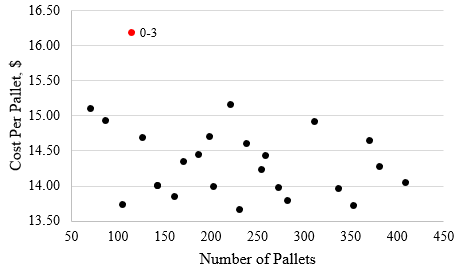
\includegraphics[width=110mm]{analysis_noPriorityCost_03.PNG}
\caption{Graph Cost per Pallet vs. Number Pallets: No Priority Cost}
\label{fig_noPriorityCost}
\end{figure}
Of note, the quantile combination of the minimum for Super/999 cargo and the 75th percentile for Priority 2/3 cargo results in the highest cost per pallet over all other demand pairings. The only visible reason for this disparity in cost is that out of the 10 aircraft allocated to ship 57 pallets to each base, two C-5s from KWRI to ETAR and 8 C-130s from KSUU to RKSO, one C-5 utilizes only 58.3\% of the pallet slots and one C-130 utilizes a mere 12.5\%. \par 
To assess stochasticity in demand, a cost frontier for the 25 cost estimates is created that accounts for an ``actual" demand that is realized post solution processing. Graphing the demand data suggests that the Super/999/1 cargo may be modeled by a uniform distribution, while the Priority 2/3 cargo follows a triangular distribution.

\begin{figure}[H]
\centering
\begin{minipage}[b]{0.4\textwidth}
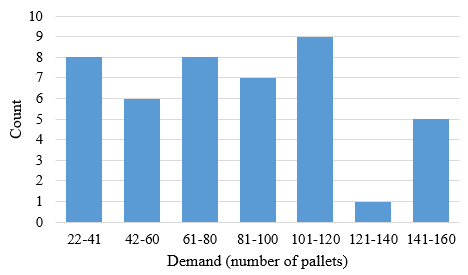
\includegraphics[width=65mm]{analysis_histogramSuper.PNG}
\caption{Histogram of Super/999/1 Cargo}
\label{fig_histogramSuper}
\end{minipage}
\hspace{10mm}
\begin{minipage}[b]{0.4\textwidth}
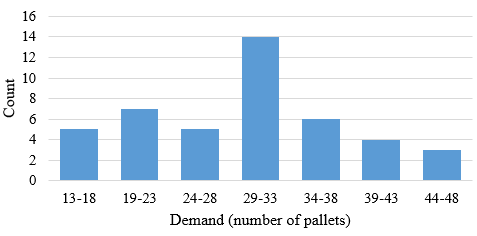
\includegraphics[width=65mm]{analysis_histogramStd.PNG}
\caption{Histogram of Priority 2/3 Cargo}
\label{fig_histogramStd}
\end{minipage}
\end{figure}
Demand distributions are created using data parameters for each of the cargo types, found in Table \ref{table_triangular}. One hundred demand samples are populated through random draws from the corresponding distributions.
\begin{table}[H]
\centering
\caption{Data Parameters per Priority Type}
\label{table_triangular}
\begin{tabular}{@{}lcc@{}}
\toprule
 & Super/999/1 & Priority 2/3 \\ \midrule
Min & 22 & 13 \\
Mode & N/A & 32 \\
Max & 155 & 49 \\ \bottomrule
\end{tabular}
\end{table}
The amount of excess and shortage of cargo of each type is calculated and multiplied by a priority cost depending on type of offense (excess or shortage) and cargo type. Several priority cost schema are used since ``real world" cost consequences are not documented for the generic cargo descriptions of Super/999/1 or Priority 2/3.  

\section{Fixed Cost Models}
Initial penalty cost models set a fix cost for shorting or exceeding the actual demand for each cargo priority type.  The first penalty cost allotment is arranged so that all penalty costs are the same. Tables \ref{table_penaltyCost1111} and \ref{table_top3_1111} depict the costs and demand combinations, respectively, for Model\refstepcounter{nc}\label{FC_1111} \ref{FC_1111}. As Table \ref{table_top3_1111} shows, the least costly demand combination given the penalty costs are all the same and at the equivalent of one kilo-pound of jet fuel, is setting the expected demand for Super/999 to the 50th percentile and Priority 2/3 to the 75th percentile.
\begin{table}[H]
\centering
\begin{minipage}[b]{0.4\textwidth}
\caption{Penalty Cost Model \ref{FC_1111}}
\label{table_penaltyCost1111}
\begin{tabular}{@{}lcc@{}}
\toprule
 & Super/999/1 & Priority 2/3 \\ \midrule
Excess & 1 & 1 \\
Short & 1 & 1 \\ \bottomrule
\end{tabular}
\end{minipage}
\hspace{10mm}
\begin{minipage}[b]{0.4\textwidth}
\caption{Top Demand Combinations for Penalty Cost Model \ref{FC_1111}: Quantile/Demand Amount}
\label{table_top3_1111}
\begin{tabular}{@{}lcc@{}}
\toprule
 & Super/999/1 & Priority 2/3 \\ \midrule
1 & 50\% / 80 & 75\% / 35 \\
2 & 25\% / 50 & 50\% / 30 \\
3 & 75\% / 106 & 75\% / 35 \\ \bottomrule
\end{tabular}
\end{minipage}
\end{table}


The second penalty cost model is arranged so that shorting Super/999/1 cargo is two times more offensive than shorting Priority 2/3 cargo and four times more offensive than exceeding Priority 2/3 cargo. With this cost model, depicted in Table \ref{table_penaltyCost1}, the three expected demand combinations with the lowest cost per pallet can be seen in Table \ref{table_top3_1}. These three combinations remain the top contenders even when the penalty costs of Model\refstepcounter{nc}\label{FC_4321} \ref{FC_4321} are all doubled.   

\begin{table}[H]
\centering
\begin{minipage}[b]{0.4\textwidth}
\caption{Penalty Cost Model \ref{FC_4321}}
\label{table_penaltyCost1}
\begin{tabular}{@{}lcc@{}}
\toprule
 & Super/999/1 & Priority 2/3 \\ \midrule
Excess & 3 & 1 \\
Short & 4 & 2 \\ \bottomrule
\end{tabular}
\end{minipage}
\hspace{10mm}
\begin{minipage}[b]{0.4\textwidth}
\caption{Top Demand Combinations for Penalty Cost Model \ref{FC_4321}: Quantile/Demand Amount}
\label{table_top3_1}
\begin{tabular}{@{}lcc@{}}
\toprule
 & Super/999/1 & Priority 2/3 \\ \midrule
1 & 50\% / 80 & 75\% / 35 \\
2 & 75\% / 106 & 75\% / 35 \\
3 & 75\% / 106 & 50\% / 30 \\ \bottomrule
\end{tabular}
\end{minipage}
\end{table}
The result of Model \ref{FC_4321} makes sense, because expecting demand to be at the 50th percentile or higher ensures that the egregious error of shorting an order is mitigated for both cargo types. This is especially true for Priority 2/3 cargo since the mode of the given data is 32, therefore expecting a demand of 35 will avoid shorting a shipment compared to assuming a demand of 30. \par
The third cost model, seen in Table \ref{table_penaltyCostTover}, places emphasis on not exceeding actual demand. The penalty cost for sending too much of a product doubles sending too little. Two of the three combinations with the least cost for Model\refstepcounter{nc}\label{FC_Tover} \ref{FC_Tover}, Tables \ref{table_penaltyCostTover} and \ref{table_top3_Tover}, differ from Model \ref{FC_4321}. The second contender in Model \ref{FC_Tover}, setting Super/999/1 cargo at the 50th percentile and Priority 2/3 at the 75th percentile, is Model \ref{FC_1111} and \ref{FC_4321}'s most economical expected demand combination. 
\begin{table}[H]
\centering
\begin{minipage}[b]{0.4\textwidth}
\caption{Penalty Cost Model \ref{FC_Tover}}
\label{table_penaltyCostTover}
\begin{tabular}{@{}lcc@{}}
\toprule
 & Super/999/1 & Priority 2/3 \\ \midrule
Excess & 2 & 2 \\
Short & 1 & 1 \\ \bottomrule
\end{tabular}
\end{minipage}
\hspace{10mm}
\begin{minipage}[b]{0.4\textwidth}
\caption{Top Demand Combinations for Penalty Cost Model \ref{FC_Tover}: Quantile/Demand Amount}
\label{table_top3_Tover}
\begin{tabular}{@{}lcc@{}}
\toprule
 & Super/999/1 & Priority 2/3 \\ \midrule
1 & 25\% / 21 & 50\% / 30 \\
2 & 50\% / 80 & 75\% / 35 \\
3 & 25\% / 21 & 25\% / 21 \\ \bottomrule
\end{tabular}
\end{minipage}
\end{table}
The fourth penalty cost model\refstepcounter{nc}\label{FC_Tshort}, Table \ref{table_penaltyCostTshort}, is the opposite of Model \ref{FC_Tover}'s; shorting demand is twice as egregious as exceeding. The same expected demand combinations for the first two are not only the same as Model \ref{FC_4321}, but also remain the same even when the fixed costs are doubled and quadrupled.
\begin{table}[H]
\centering
\begin{minipage}[b]{0.4\textwidth}
\caption{Penalty Cost Model \ref{FC_Tshort}}
\label{table_penaltyCostTshort}
\begin{tabular}{@{}lcc@{}}
\toprule
 & Super/999/1 & Priority 2/3 \\ \midrule
Excess & 1 & 1 \\
Short & 2 & 2 \\ \bottomrule
\end{tabular}
\end{minipage}
\hspace{10mm}
\begin{minipage}[b]{0.4\textwidth}
\caption{Top Demand Combinations for Penalty Cost Model \ref{FC_Tshort}: Quantile/Demand Amount}
\label{table_top3_Tshort}
\begin{tabular}{@{}lcc@{}}
\toprule
 & Super/999/1 & Priority 2/3 \\ \midrule
1 & 50\% / 80 & 75\% / 35 \\
2 & 75\% / 106 & 75\% / 35 \\
3 & 100\% / 155 & 25\% / 21 \\ \bottomrule
\end{tabular}
\end{minipage}
\end{table}
 Presuming the assumption of distributions for the cargo types is correct, setting expected demand to the 50th percentile for Super/999/1 cargo and to the 75th percentile for Priority 2/3 cargo is a preference in the fixed cost models. 
\section{Variable Cost Models}
The original pallet cost is the fuel amount required to fly aircraft with a specified cargo amount from a source to a destination and return to the source empty. Taking into consideration that under-shipping or over-shipping an item may require back-filling an order or returning the overage amount, respectively, the penalty cost can be viewed as a percentage of the cost to transport the pallet. The penalty cost could be the full pallet cost to account for a back-order or a range of percentages to account for the return of the pallet. The portion of flight costs associated with transporting cargo ranges from approximately 50 to 57 percent.\par
Setting the penalty cost amount to 100 percent for all cargo grievances for Model\refstepcounter{nc}\label{PC_100} \ref{PC_100} results in the least costly demand combinations for pallet costs, as seen in Table \ref{table_top3_PC100}, differing from their original penalty-free costs by only approximately four percent and the most costly by almost 160 percent. Figure \ref{fig_GraphNoPriorityCost} shows the effect of penalty costs on the cost per pallet when all penalty costs are equal to the original cost per pallet.  
\begin{table}[H]
    \centering
    \caption{Top Demand Combinations for Penalty Cost Model \ref{PC_100}: Quantile/Demand Amount}
    \label{table_top3_PC100}
    \begin{tabular}{@{}lcc@{}}
    \toprule
        & Super/999/1 & Priority 2/3 \\ \midrule
        1 & 25\% / 50 & 50\% / 30 \\
        2 & 25\% / 50 & 25\% / 21 \\
        3 & 25\% / 50 & 75\% / 35 \\ \bottomrule
    \end{tabular}
\end{table}

\begin{figure}[H]
\centering
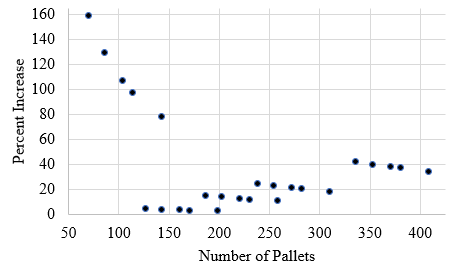
\includegraphics[width=105mm]{analysis_percent_100.PNG}
\caption{Graph Percentage Increase of Cost per Pallet vs. Number Pallets: Cost Model \ref{PC_100} (100\% Penalty)}
\label{fig_GraphNoPriorityCost}
\end{figure}

Keeping the shortage penalty constant at 100\% of the pallet cost, the final cost per pallet of the top (least costly) three demand combinations for the different proportional overage penalties are shown in Figure \ref{fig_GraphAllPercent}. Final cost per pallet does not strictly increase with an increase of penalty cost due to a shift in expected demand. Figure \ref{fig_Graph_PercentQuantiles} depicts the demand percentile of the foremost least costly demand combination over the different variable overage penalty costs. From this figure, there is a distinct expected demand quantile for each cargo type that results in the lowest total cost per pallet with a stochastic realized demand. In this instance, the expected demand quantity for a majority of the range of costs are the 75th percentile for Super/999/1 cargo and the 50th percentile for Priority 2/3 cargo.     

\begin{figure}[H]
\centering
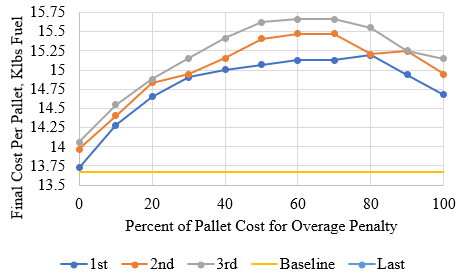
\includegraphics[width=105mm]{analysis_percent_All_Top3.PNG}
\caption{Graph Cost per Pallet vs Percentage of Pallet Cost for Overage Penalty}
\label{fig_GraphAllPercent}
\end{figure}

\begin{figure}[H]
\centering
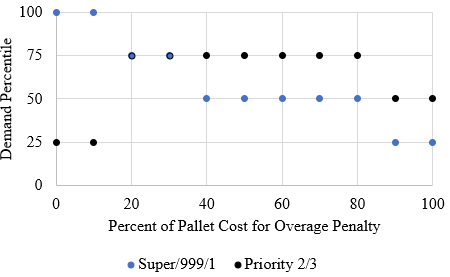
\includegraphics[width=105mm]{analysis_percent_Quantiles.PNG}
\caption{Graph Top Demand Percentile vs Percent of Pallet Cost for Overage Penalty}
\label{fig_Graph_PercentQuantiles}
\end{figure}

\section{Aircraft Allocation}
One finding with the notional example is that no C-17s were allocated to transport cargo from CONUS to the chosen OCONUS bases of Ramstein AB and Osan AB. This is likely due to the similar fuel efficiency between the C-5 and C-17 and that the C-5 has a higher cargo throughput compared to the C-17 when not accounting for mission capable rates \cite{Reiman2014}. Figure \ref{fig_numAircraft} depicts the number of aircraft allocated to fly for a given number of pallets.  Due to the lighter pallet weight of 2.6 Klbs, the C-130 is more fuel efficient compared to the C-17 and C-5.
%stupid column chart would not work, couldn't alter the ridiculous horizontal axis bounds because it thought it was categorical. Made scatter plot instead and added lines because it makes it easier to see where things are vs No-lines, but dimmed the lines to it's possibly more clear that the points are more important to note??? 
\begin{figure}[H]
\centering
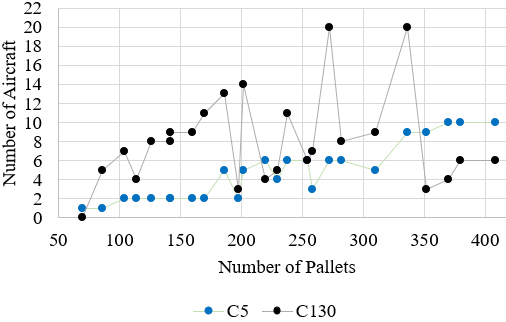
\includegraphics[width=105mm]{analysis_numC5andC130.PNG}
\caption{Graph Number of Aircraft vs Number of Pallets}
\label{fig_numAircraft}
\end{figure}

\textcolor{red}{Add figure of Costs vs Num Pallets with solely using each MDS}


%___________________________________
%Chapter 5 -- Conclusion
 \chapter{Conclusions and Future Research}\label{ch5}
  \section{Conclusion}
This research is a proof of concept that given stochastic demand, there is a given expected amount that minimizes penalty costs depending on the cost profile. 

%Appendix Section
%___________________________________
\appendix
	\chapter{Visual Basic for Applications Code}\label{A01_VBA}
		\lstloadlanguages{VBScript}
\lstset{language=VBScript,
		basicstyle=\smaller[2],
		commentstyle=\rmfamily\smaller,
  		showstringspaces=false,
  		xleftmargin=4ex,literate={<-}{{$\leftarrow$}}1 {~}{{$\sim$}}1}
\lstset{escapeinside={(*}{*)}} 


\section{Fuel} \label{code_fuel}
\begin{lstlisting}
Option Explicit
Public plane, C5, C17, C130, fromBase, toBase As Long
Public selectMDS As String

Function fuelCalculations(selectMDS, distance, Payload, numStops)
'Find the cost of fuel for the max payload
    Dim specRange, wgross, gwForMaxDist, fuel, wff, wfc, wfd, A, B, C, D, _
    fuelReq, myAnswer As Double
    Dim i, j, num As Long
    Dim plane, wop, wgmt, wmaxfuel, wpmax, wfrah, wfstto, wfapp, wp, alt As Double
    Dim distRange, climb, cruise, descent, given As Range
    
    Set distRange = Range("rangeBeta")
    Set cruise = Range("cruiseBeta")
    Set climb = Range("climbBeta")
    Set descent = Range("descentBeta")
    Set given = Range("GivensTable")
    
    plane = getPlane(selectMDS)
    
    'for ease of reading the equations.
    wop = given(plane, 2)
    wgmt = given(plane, 3)
    wpmax = given(plane, 5)
    wfrah = given(plane, 6)
    wfstto = given(plane, 7)
    wfapp = given(plane, 8)
    alt = given(plane, 9)
    
    wmaxfuel = wgmt - wop - wfrah - Payload
    If wmaxfuel + wfrah > given(plane, 4) Then wmaxfuel = given(plane, 4) - wfrah
    wgross = wop + Payload + wmaxfuel + wfrah 'gross takeoff weight
    num = numStops + 1

    'A-D are used in the fuelConsumed Function, found under Equation 23 from
    'Reiman 2014 page 52
    A = cruise(plane, 6) / 3
    B = cruise(plane, 5) / 2 + cruise(plane, 6) * (wop + wfrah + Payload) + _
    (cruise(plane, 7) / 2) * alt
    C = cruise(plane, 2)+cruise(plane, 3)*alt+cruise(plane, 4)*(alt)^2 + _
        cruise(plane, 5) * (wop + wfrah + Payload) + _
        cruise(plane, 6) * (wop + wfrah + Payload)^ 2 + _
        cruise(plane, 7) * alt * (wop + wfrah + Payload)
    D = -distance / num
    
    wff = fuelConsumed(A, B, C, D)
    
    'Equation 19 and 20 from Reiman 2014 page 50
    wfc = climb(plane, 2) + climb(plane, 3) * alt + climb(plane, 4) * (alt)^ 2 + _
          climb(plane, 5) * (alt) ^ 3 + climb(plane, 6) * wgross + _
          climb(plane, 7) * (wgross) ^ 2 + climb(plane, 8) * (wgross) ^ 3 + _
          climb(plane, 9) * 10 ^ (-6) * (alt) ^ 2 * (wgross)^ 3 + _
          climb(plane, 10) * 10 ^ (-6) * (alt) ^ 2 * (wgross)^ 3
    wfd = descent(plane, 2)+descent(plane, 3)*(wgross-wfc-wff-wfstto) + _
          descent(plane, 4)*(wgross-wfc-wff-wfstto)^ 2 + descent(plane, 5)*alt + _
          descent(plane, 6) * alt * (wgross - wfc - wff - wfstto)
    
    fuel = num * (wff + wfc + wfd)
     
    fuelCalculations = fuel
End Function

'this function returns the Klbs fuel consumed during the cruise portion of flight
Function fuelConsumed(A, B, C, D) As Double
    Dim commonTerm1, commonTerm2, cubeRoot1, cubeRoot2 As Double
    
    commonTerm1 = 2# * (B ^ 3) - 9# * A * B * C + 27# * (A^ 2) * D
    commonTerm2 = 4 * ((B ^ 2) - 3 * A * C)^ 3
    cubeRoot1 = 0.5 * (commonTerm1 + Sqr((commonTerm1^ 2) - commonTerm2))
    cubeRoot2 = 0.5 * (commonTerm1 - Sqr((commonTerm1^ 2) - commonTerm2))
    
        If (cubeRoot1 < 0) Then
            cubeRoot1 = -(-cubeRoot1)^ (1 / 3)
        Else
            cubeRoot1 = (cubeRoot1^ (1 / 3))
        End If
    
        If (cubeRoot2 < 0) Then
            cubeRoot2 = -(-cubeRoot2)^ (1 / 3)
        Else
            cubeRoot2 = (cubeRoot2^ (1 / 3))
            End If
    
        '//g=-B/3A
        '//  -1/3A(1/2 [2B^3-9ABC+27A^2 D+v((2B^3-9ABC+27A^2 D)^2-4(B^2-3AC)^3)])
        '//  -1/3A(1/2 [2B^3-9ABC+27A^2 D-v((2B^3-9ABC+27A^2 D)^2-4(B^2-3AC)^3)])
        
        fuelConsumed = (-B/(3*A)) - (1/(3*A)) * cubeRoot1 - (1/(3*A)) * cubeRoot2

End Function

'This function facilitates the fuel costs (accounts for multiple enroute stops) 
Function fuel(selectMDS, distance, Payload)
    Dim numberStops As Long
    numberStops = numStops(selectMDS, distance, Payload)
    fuel = fuelCalculations(selectMDS, distance, Payload, numberStops)
End Function
\end{lstlisting}
\Section{Distance}
\begin{lstlisting}
'Calculates the vincenty elliptical great circle geodetic curve 
'(Code courtesy of Mike Gavaghan)
Function vincentyDistance(lat1, long1, lat2, long2) As Double
    'Ellipsoid properties based on WGS-84
    Dim semiMajor, inverseFlattening, flattening, semiMinor, A, B, big_A, big_B, _
    f, TwoPi, phi1, phi2, lambda, lambda1, lambda2, a2b2b2, tanphi1, tanU1, U1, _
    sinU1 As Double
    Dim cosU1, tanphi2, tanU2, U2, small_u2, sinU2, cosU2, sinU1sinU2, _
    cosU1sinU2, sinU1cosU2, cosU1cosU2, a2, b2, omega, i, s As Double
    Dim sigma, deltasigma, lambda0, sinlambda, coslambda, sin2sigma, sinsigma, _
    cossigma, sinalpha, alpha, cosalpha, cos2alpha, cos2sigmam, cossigmam, _
    cos2sigmam2, C  As Double
    Dim converged As Boolean
    Dim change As Variant
        
        semiMajor = 6378137#   'Meters
        inverseFlattening = 298.257223563
        flattening = 1# / inverseFlattening
        semiMinor = (1# - flattening) * semiMajor
        
        Application.ScreenUpdating = False

    'simplify
        A = semiMajor
        B = semiMinor
        f = flattening
        TwoPi = 2# * Application.Pi

    'get parameters as radians
        phi1 = lat1 * Application.Pi / 180#
        lambda1 = long1 * Application.Pi / 180#
        phi2 = lat2 * Application.Pi / 180#
        lambda2 = long2 * Application.Pi / 180#

    'calculations
        a2 = A * A
        b2 = B * B
        a2b2b2 = (a2 - b2) / b2

        omega = lambda2 - lambda1

        tanphi1 = Tan(phi1)
        tanU1 = (1# - f) * tanphi1
        U1 = Atn(tanU1)
        sinU1 = Sin(U1)
        cosU1 = Cos(U1)
    
        tanphi2 = Tan(phi2)
        tanU2 = (1# - f) * tanphi2
        U2 = Atn(tanU2)
        sinU2 = Sin(U2)
        cosU2 = Cos(U2)
    
        sinU1sinU2 = sinU1 * sinU2
        cosU1sinU2 = cosU1 * sinU2
        sinU1cosU2 = sinU1 * cosU2
        cosU1cosU2 = cosU1 * cosU2

    'eq. 13
        lambda = omega

    'intermediates we'll need to compute 's'
    
        big_A = 0#
        big_B = 0#
        sigma = 0#
        deltasigma = 0#
        converged = False

    For i = 0 To 20
        lambda0 = lambda

        sinlambda = Sin(lambda)
        coslambda = Cos(lambda)

        'eq. 14
        sin2sigma = (cosU2 * sinlambda * cosU2 * sinlambda) + _
        (cosU1sinU2 - sinU1cosU2 * coslambda) ^ 2
        sinsigma = Sqr(sin2sigma)

        'eq. 15
        cossigma = sinU1sinU2 + (cosU1cosU2 * coslambda)

        'eq. 16
        sigma = Application.Atan2(cossigma, sinsigma)

        'eq. 17    Careful!  sin2sigma might be almost 0!
         If sin2sigma = 0 Then sinalpha = 0 Else sinalpha = _
                                                cosU1cosU2 * sinlambda / sinsigma
        Dim check As Variant
        check = sigma * 2
        alpha = Application.Asin(sinalpha)
        cosalpha = Cos(alpha)
        cos2alpha = cosalpha * cosalpha

        'eq. 18    Careful!  cos2alpha might be almost 0!
        If cos2alpha = 0# Then cos2sigmam = 0# Else cos2sigmam = _
                                            cossigma - 2 * sinU1sinU2 / cos2alpha
        small_u2 = cos2alpha * a2b2b2

        cos2sigmam2 = cos2sigmam * cos2sigmam

        'eq. 3
        big_A = 1+small_u2/16384*(4096+small_u2*(-768+small_u2*(320-175*small_u2)))

        'eq. 4
        big_B = small_u2/1024*(256+small_u2*(-128+small_u2*(74-47*small_u2)))

        'eq. 6
        deltasigma = big_B*sinsigma*(cos2sigmam+big_B / 4*(cossigma * _
        (-1+2*cos2sigmam2)-big_B/6*cos2sigmam*(-3+4*sin2sigma)*(-3+4*cos2sigmam2)))

        'eq. 10
        C = f / 16 * cos2alpha * (4 + f * (4 - 3 * cos2alpha))

        'eq. 11 (modified)
        lambda = omega+(1-C)*f*sinalpha*(sigma+C*sinsigma*(cos2sigmam+C*cossigma* _
                                                                (-1+2*cos2sigmam2)))

        'see how much improvement we got
        change = Math.Abs((lambda - lambda0) / lambda)

        If i > 1 And change < 0.0000000000001 Then
            converged = True
            Exit For
        End If
    Next
    
    'eq. 19
    s = B * big_A * (sigma - deltasigma)
    
    vincentyDistance = s / 1852

End Function

' Given the altitude in 1,000s of feet, Klbs reserve, alternate and holding (rah) fuel,
'Klbs payload, Klbs fuel consumed (max fuel after payload) in Klbs,
'determines the max distance possible
Function maxDistance(selectMDS, Payload) As Double
   Dim wop, wgmt, wmaxfuel, wpmax, wfrah, wfstto, wfapp, alt, A, B, C, G, _
   totalFuelConsumed As Double
   Dim cruise, climb, descent, given As Range
    
    Set cruise = Range("cruiseBeta")
    Set climb = Range("climbBeta")
    Set descent = Range("descentBeta")
    Set given = Range("GivensTable")
    
    maxDistance = 0
    plane = getPlane(selectMDS)
    
    'for ease of reading the equations.
    wop = given(plane, 2)
    wgmt = given(plane, 3)
    wmaxfuel = given(plane, 4)
    wpmax = given(plane, 5)
    wfrah = given(plane, 6)
    wfstto = given(plane, 7)
    wfapp = given(plane, 8)
    alt = given(plane, 9)
    
   'difference from max gross takeoff and payload and reserve
    totalFuelConsumed = wgmt - wop - Payload - wfrah 
    
    If totalFuelConsumed+wfrah > wmaxfuel Then totalFuelConsumed = wmaxfuel-wfrah
    
'Use Formula distance = A*g^3 + B*g^2 + C*g coefficients. G represents fuel consumed.
    A = cruise(plane, 6)/3
    B = cruise(plane, 5)/2+cruise(plane, 6)*(wop+Payload+wfstto+wfapp+wfrah)+ _
    cruise(plane, 7) * (alt) / 2# '(ß_3/2+ß_4*(EW+w)+ß_5/2*Alt)
    C = cruise(plane, 2) + cruise(plane, 3) * alt + cruise(plane, 4) * (alt) ^ 2 + _
            cruise(plane, 5) * (wop + Payload + wfstto + wfapp + wfrah) + _
            cruise(plane, 6) * (wop + Payload + wfstto + wfapp + wfrah) ^ 2 + _
            cruise(plane, 7) * alt * (wop + Payload + wfstto + wfapp + wfrah)
    '(ß_0+ß_1*Alt+ß_2*A?lt?^2+ß_3*(EW+w)+ß_4*(EW+w)^2+ß_5*Alt*(EW+w))
    G = totalFuelConsumed

    maxDistance = A * ((G) ^ 3) + B * ((G) ^ 2) + C * G
End Function

'calculates the number of stops required for an MDS given the distance and payload
Function numStops(selectMDS, distance, Payload) As Double
    Dim stopDist As Double

    stopDist = maxDistance(selectMDS, Payload)
    numStops = distance / stopDist
    numStops = Application.WorksheetFunction.RoundDown(numStops, 0)
End Function

'given source and destination ICAOs this function finds the associated lats and longs
'and returns the distance between them
Function myDistance(fromString, toString) As Double

    Dim rowCount, colCount, aircraftCount, totalFromBases, totalToBases, totalNumAircraft, _
    i, k, col As Long
    Dim tempstring, fromPCN, toPCN As String
    Dim lat1, lat2, long1, long2, Payload, distance, baseFuel, maxpayload As Double
    Dim endCond As Boolean
    
    'Find lat/long data for "from base
    For i = 1 To 5342
        If Sheets("AirfieldData").Cells(i, 2) = fromString Then
            lat1 = Sheets("AirfieldData").Cells(i, 3)
            long1 = Sheets("AirfieldData").Cells(i, 4)
            'fromPCN = Sheets("AirfieldData").Cells(i, 7)
            Exit For
        End If
    Next
        
    'Find the lat/long for the "to" base
    For i = 1 To 5342
        If Sheets("AirfieldData").Cells(i, 2) = toString Then
            lat2 = Sheets("AirfieldData").Cells(i, 3)
            long2 = Sheets("AirfieldData").Cells(i, 4)
            'toPCN = Sheets("AirfieldData").Cells(i, 7)
            Exit For
        End If
    Next i
    
    'Populate distance
    myDistance = vincentyDistance(lat1, long1, lat2, long2)
                     
End Function
\end{lstlisting}
\Section{Pre-Processing} \label{code_preprocessing}
\begin{lstlisting}
'this sub moves through all the source and destination combinations and populates 
'the Aircraft sheet with the distance between them, fuel cost per payload pound, 
'and basic fuel cost given the aircraft MDS
Sub getDistance()
    Dim rowCount, colCount, aircraftCount, totalFromBases, totalToBases, _
    totalNumAircraft, i, k, col As Long
    Dim fromString, toString, tempstring, fromPCN, toPCN As String
    Dim lat1, lat2, long1, long2, Payload, distance, baseFuel, maxpayload, _
    payloadFuel As Double
    Dim endCond As Boolean
    
    Application.ScreenUpdating = False
    rowCount = 0
    colCount = 0
    aircraftCount = 0
    Payload = 0
    
    Do While endCond = False
        tempstring = Sheets("SupplyBases").Cells(rowCount + 2, 1)
        If IsEmpty(tempstring) Then
            endCond = True
            Exit Do
        End If
        rowCount = rowCount + 1
    Loop
    
    totalFromBases = rowCount
    endCond = False
    Do While endCond = False
        tempstring = Sheets("DemandBases").Cells(colCount + 2, 1)
       If IsEmpty(tempstring) Or tempstring = "" Then
            endCond = True
            Exit Do
        End If
        colCount = colCount + 1
    Loop
    
    totalToBases = colCount
    
    endCond = False
    Do While endCond = False
        tempstring = Sheets("Aircraft").Cells(aircraftCount + 8, 1)
       If IsEmpty(tempstring) Or tempstring = "" Then
            endCond = True
            Exit Do
        End If
        aircraftCount = aircraftCount + 1
    Loop
        
    totalNumAircraft = aircraftCount
    col = 1
     
     Application.ScreenUpdating = False
    For rowCount = 1 To totalFromBases
        fromString = Sheets("SupplyBases").Cells(rowCount + 1, 1)
        'Find lat/long data for "from base
        For i = 1 To 5342
            If Sheets("AirfieldData").Cells(i, 2) = fromString Then
                lat1 = Sheets("AirfieldData").Cells(i, 3)
                long1 = Sheets("AirfieldData").Cells(i, 4)
                fromPCN = Sheets("AirfieldData").Cells(i, 7)
                Exit For
            End If
        Next
        
        'Find the lat/long for the "to" base
        For colCount = 1 To totalToBases
            toString = Sheets("DemandBases").Cells(colCount + 1, 1)
            If Not toString = fromString Then
                For i = 1 To 5342
                    If Sheets("AirfieldData").Cells(i, 2) = toString Then
                        lat2 = Sheets("AirfieldData").Cells(i, 3)
                        long2 = Sheets("AirfieldData").Cells(i, 4)
                        toPCN = Sheets("AirfieldData").Cells(i, 7)
                        Exit For
                    End If
                    Sheets("Aircraft").Cells(6, 14 + col) = fromString
                    Sheets("Aircraft").Cells(7, 14 + col) = toString
                    Sheets("maxfuel").Cells(1, 1 + col) = fromString
                    Sheets("maxfuel").Cells(2, 1 + col) = toString
                    Sheets("basefuel").Cells(1, 1 + col) = fromString
                    Sheets("basefuel").Cells(2, 1 + col) = toString
                
                Next i
                
                'Populate distance and fuel cost/(payload Klb) given aircraft type for all 
                'aircraft on "aircraft" sheet
                distance = vincentyDistance(lat1, long1, lat2, long2)
                For k = 1 To totalNumAircraft
                    selectMDS = Sheets("Aircraft").Cells(k + 7, 2).Value
                    Payload = Sheets("Aircraft").Cells(k + 7, 6).Value
                    maxpayload = Sheets("Aircraft").Cells(k + 7, 6).Value
                    
                    Sheets("Aircraft").Cells(k+7, 14).Value = _
                                                        Sheets("Aircraft").Cells(k+7, 1)
                    Sheets("maxfuel").Cells(k+2, 1).Value = _
                                                        Sheets("Aircraft").Cells(k+7, 1)
                    Sheets("basefuel").Cells(k+2, 1).Value = _ 
                                                        Sheets("Aircraft").Cells(k+7, 1)
                    
                     Sheets("Aircraft").Cells(k + 7, 13 + col + 1).Value = distance
                     'Sheets("Aircraft").Cells(k + 3, 14 + col).Value = _
                     airfieldNodalReduction(selectMDS, lat1, long1, lat2, long2, _
                     fromPCN, toPCN, payload)
                     baseFuel = fuel(selectMDS, distance, 0)
                     payloadFuel = fuel(selectMDS, distance, Payload)
                     
                     Sheets("maxfuel").Cells(k + 2, 1 + col).Value = _
                     (payloadFuel - baseFuel) / maxpayload
                     
                     Sheets("basefuel").Cells(k + 2, 1 + col).Value = baseFuel
                Next k
                col = col + 1
            End If
        Next colCount
        
    Next rowCount
Application.ScreenUpdating = True
End Sub

\end{lstlisting}

\section{Post Processing}
\begin{lstlisting}
Sub FinalCost()
    Dim endCond As Boolean
    Dim tempstring, toString, fromString, planeString As String
    Dim aircraftCount, allocatedCount, baseCount, i, j, k As Long
    Dim distance, Payload As Double
      
     aircraftCount = 0
     allocatedCount = 0
     baseCount = 0
     
     Application.ScreenUpdating = False
    
    'count the number of aircraft
    endCond = False
    Do While endCond = False
        tempstring = Sheets("Aircraft").Cells(aircraftCount + 8, 1)
       If IsEmpty(tempstring) Or tempstring = "" Then
            endCond = True
            Exit Do
        End If
        aircraftCount = aircraftCount + 1
    Loop
    
    'count the number of allocated aircraft
    endCond = False
    Do While endCond = False
        tempstring = Sheets("ACAllocation").Cells(1, allocatedCount + 3)
       If IsEmpty(tempstring) Or tempstring = "" Then
            endCond = True
            Exit Do
        End If
        allocatedCount = allocatedCount + 1
    Loop
    
   'count the number of bases
    endCond = False
    Do While endCond = False
        tempstring = Sheets("ACAllocation").Cells(baseCount + 2, 1)
       If IsEmpty(tempstring) Or tempstring = "" Then
            endCond = True
            Exit Do
        End If
        baseCount = baseCount + 1
    Loop
    
    For i = 1 + 1 To baseCount + 1 'go down the rows of bases
        fromString = Sheets("ACAllocation").Cells(i, 1)
        toString = Sheets("ACAllocation").Cells(i, 2)
        For j = 1 + 2 To allocatedCount + 3 'go across the columns of allocated
            planeString = Sheets("ACAllocation").Cells(1, j)
            For k = 1 To aircraftCount 'loop through the total aircraft
                tempstring = Sheets("Aircraft").Cells(k + 7, 1)
                If planeString = tempstring And _ 
                                 Sheets("ACAllocation").Cells(i, j) > 0 Then
                            selectMDS = Sheets("Aircraft").Cells(k + 7, 2).Value
                    distance = myDistance(fromString, toString)
                    Payload = Sheets("FinalPayload").Cells(i, j).Value
                    Sheets("finalFuel").Cells(1, j) = planeString
                    Sheets("finalFuel").Cells(i, 1) = fromString
                    Sheets("finalFuel").Cells(i, 2) = toString
                    'cycle cost is payload to destination, empty back
                    Sheets("finalFuel").Cells(i, j) = _
                        fuel(selectMDS, distance, Payload)+fuel(selectMDS, distance, 0)
                    Exit For
                End If
            Next k
        Next j
    Next i
    Application.ScreenUpdating = True
End Sub
\end{lstlisting}
	\chapter{General Algebraic Modeling System Code}\label{A02_GAMS}
		\begin{lstlisting}
Sets
  i supply bases
  j demand bases
  k item types /super, standard/
  l aircraft
  c index for climb /0*8/
  ws given weights;

Parameters
   Ed(j,k)       expected demand at base j for item k
   s(i,k)        supply inventory at base i of item k
   w(k)          weight of item k
   h(j,k)        holding cost ($) at base j of item k
   p(j,k)        penalty for shorting demand at base j of item k
   alt(l)        the altitude of aircraft l
   wg(l,ws)      weight parameters of aircraft l

   maxFuel(l,i,j) fuel to fly the max payload for distance i j and acrft
   baseFuel(l,i,j);

$onecho > taskout.txt
Set = i          rng=SupplyBases!a1          rdim=1
Set = j          rng=DemandBases!a1                 rdim=1
Set= l           rng=Aircraft!a8      rdim=1
Set=ws           rng=Aircraft!b7:K7            cdim=1 IgnoreColumns=B
Par=w            rng=Items!b2         rdim=1
Par = wg         rng=Aircraft!a7      rdim=1  cdim=1 IgnoreColumns=B
Par= maxFuel     rng=maxfuel!a1      rdim=1 cdim=2
Par=baseFuel     rng=basefuel!a1     rdim=1 cdim=2
$offecho

$call GDXXRW indata_solve2.xlsm trace=3 @taskout.txt
$GDXIN indata_solve2.gdx
$LOADDC i j l ws wg maxFuel baseFuel
$GDXIN

Variables
  z           objective function value;

z.lo=0;
z.up=100000;

Positive Variables
wp(i,j,l)     payload weight for route i to j on aircraft l
x(i,j,k,l)   number of pallets from i to j of item k to fly on aircraft l  ;
wp.up(i,j,l)=270; #maximum payload weight of C5
x.up(i,j,k,l)=36;

Binary Variables
  y(i,j,l)     1 if from base i to base j aircraft l is assigned to deliver something

Equations
  objfun                    defines the overall objective function
  meetexpdemand(j,k)        Must meet expected demand
  payloadWeightbound(i,j,l) cannot exceed aircraft weight capacity
  spacebound(i,j,l)         cannot exceed aircraft floor space capacity
  oneassignmentperac(l)     only assign an aircraft to one i-j combination
*  supply(i,k)               cannot exceed available supply
  payload(i,j,l)            payload weight;

objfun.. z=e=  1*sum(i,sum(j,sum(l,(maxFuel(l,i,j)*wp(i,j,l)+
baseFuel(l,i,j))*y(i,j,l))));

************************Constraints************************
meetexpdemand(j,k)..         sum(i,sum(l,x(i,j,k,l))) =e= Ed(j,k);
payloadWeightbound(i,j,l)..  w('super')*x(i,j,'super',l)+
    w('standard')*x(i,j,'standard',l) =l= wg(l,'wapmax')*y(i,j,l);
spacebound(i,j,l)..          x(i,j,'super',l)+
                     x(i,j,'standard',l)=l= wg(l,'scap')*y(i,j,l);
oneassignmentperac(l)..      sum(i,sum(j,y(i,j,l))) =l= 1;
payload(i,j,l)..             wp(i,j,l)=e=w('super')*x(i,j,'super',l)+
                                    w('standard')*x(i,j,'standard',l)

Model MausModel / all /;

Ed('ETAR','super')=22;  Ed('ETAR','standard')=7;
Ed('RKSO','super')=22;  Ed('RKSO','standard')=7;

w('super')=2.6; w('standard')=2.6;

option nlp=minos;
option minlp=baron;

Solve MausModel minimizing z using minlp;

execute_unload 'indata_solve2.gdx', x,y,wp, z, wg;
execute 'gdxxrw.exe indata_solve2.gdx O=indata_solve2.xlsm var= 
x.l rng=CargoAllocation!a1' ;
execute 'gdxxrw.exe indata_solve2.gdx O=indata_solve2.xlsm var=
y.l rng=ACAllocation!a1' ;
execute 'gdxxrw.exe indata_solve2.gdx O=indata_solve2.xlsm var=
wp.l rng=FinalPayload!a1' ;;
execute 'gdxxrw.exe indata_solve2.gdx O=indata_solve2.xlsm var=
z.l rng=GAMScost!a1' ;
\end{lstlisting}


%Bibliography
%%___________________________________
\backmatter
	\singlespace
    \Urlmuskip=0mu plus 1mu\relax
    \raggedright
\bibliographystyle{ieeetr}
	\bibliography{litReview.bib} 
	\clearpage
    \pagebreak
  %  \date{March 2013}
\ReportDate{10--02--2013} \ReportType{Master's Thesis}
\DatesCovered{Sept 2011 --- Mar 2013}

\Title{\centering \MakeUppercase{AFIT/ENP Thesis Primer:}\\
                  \MakeUppercase{ a document in \LaTeX}}

%\Title{\centering \MakeUppercase{Evaluation of Interplanetary
%Magnetic Field Tracing Models Using Impulsive SEP's}}

%\ContractNumber{DACA99--99--C--9999}

%\GrantNumber{}
%\ProgramElementNumber{}
%\ProjectNumber{09ENP???}
%\TaskNumber{}
%\WorkUnitNumber{}

\Author{Amy L. Magnus}

\PerformingOrg{Air Force Institute of Technology\\[-1pt]
    Graduate School of Engineering and Management (AFIT/EN)\\[-1pt]
    2950 Hobson Way\\[-1pt]
    WPAFB OH 45433-7765}

\POReportNumber{AFIT/GAP/ENP/11-S01}

\SponsoringAgency{Department of Engineering Physics\\[-1pt]
2950 Hobson Way\\[-1pt]
WPAFB OH 45433-7765\\[-1pt]
DSN 271-0690, COMM 937-255-3636\\[-1pt]
Email: amy.magnus@afit.edu }

\Acronyms{AFWA}
%\SMReportNumber{}
\DistributionStatement{DISTRIBUTION STATEMENT A:\\
\MakeUppercase{Approved for Public Release; distribution unlimited.}}

\Abstract{This primer aids the AFIT student in generating the first draft of
their thesis using \Latex. The primer is produced according the tenets
described within the document.  All source code is provided in a zip
file posted to \primerAddress.  The file structure of this zip file
demonstrates a practical way to organize a thesis with its supporting
materials and---further---illustrates how your document can be produced
with version control.
}

\SubjectTerms{LaTeX,Thesis,typesetting}

\NumberPages{27}
%\ReportClassification{}
%\PageClassification{}
%\AbstractClassification{}
\AbstractLimitation{U}

\ResponsiblePerson{Dr. I. M. Smart, AFIT/ENP}

\RPTelephone{(937) 255-3636, x4555; amy.magnus@afit.edu}

\MakeRptDocPage


    
\end{document}